% Options for packages loaded elsewhere
\PassOptionsToPackage{unicode}{hyperref}
\PassOptionsToPackage{hyphens}{url}
\PassOptionsToPackage{dvipsnames,svgnames,x11names}{xcolor}
%
\documentclass[
  letterpaper,
  DIV=11,
  numbers=noendperiod]{scrartcl}

\usepackage{amsmath,amssymb}
\usepackage{iftex}
\ifPDFTeX
  \usepackage[T1]{fontenc}
  \usepackage[utf8]{inputenc}
  \usepackage{textcomp} % provide euro and other symbols
\else % if luatex or xetex
  \usepackage{unicode-math}
  \defaultfontfeatures{Scale=MatchLowercase}
  \defaultfontfeatures[\rmfamily]{Ligatures=TeX,Scale=1}
\fi
\usepackage{lmodern}
\ifPDFTeX\else  
    % xetex/luatex font selection
\fi
% Use upquote if available, for straight quotes in verbatim environments
\IfFileExists{upquote.sty}{\usepackage{upquote}}{}
\IfFileExists{microtype.sty}{% use microtype if available
  \usepackage[]{microtype}
  \UseMicrotypeSet[protrusion]{basicmath} % disable protrusion for tt fonts
}{}
\makeatletter
\@ifundefined{KOMAClassName}{% if non-KOMA class
  \IfFileExists{parskip.sty}{%
    \usepackage{parskip}
  }{% else
    \setlength{\parindent}{0pt}
    \setlength{\parskip}{6pt plus 2pt minus 1pt}}
}{% if KOMA class
  \KOMAoptions{parskip=half}}
\makeatother
\usepackage{xcolor}
\setlength{\emergencystretch}{3em} % prevent overfull lines
\setcounter{secnumdepth}{-\maxdimen} % remove section numbering
% Make \paragraph and \subparagraph free-standing
\makeatletter
\ifx\paragraph\undefined\else
  \let\oldparagraph\paragraph
  \renewcommand{\paragraph}{
    \@ifstar
      \xxxParagraphStar
      \xxxParagraphNoStar
  }
  \newcommand{\xxxParagraphStar}[1]{\oldparagraph*{#1}\mbox{}}
  \newcommand{\xxxParagraphNoStar}[1]{\oldparagraph{#1}\mbox{}}
\fi
\ifx\subparagraph\undefined\else
  \let\oldsubparagraph\subparagraph
  \renewcommand{\subparagraph}{
    \@ifstar
      \xxxSubParagraphStar
      \xxxSubParagraphNoStar
  }
  \newcommand{\xxxSubParagraphStar}[1]{\oldsubparagraph*{#1}\mbox{}}
  \newcommand{\xxxSubParagraphNoStar}[1]{\oldsubparagraph{#1}\mbox{}}
\fi
\makeatother


\providecommand{\tightlist}{%
  \setlength{\itemsep}{0pt}\setlength{\parskip}{0pt}}\usepackage{longtable,booktabs,array}
\usepackage{calc} % for calculating minipage widths
% Correct order of tables after \paragraph or \subparagraph
\usepackage{etoolbox}
\makeatletter
\patchcmd\longtable{\par}{\if@noskipsec\mbox{}\fi\par}{}{}
\makeatother
% Allow footnotes in longtable head/foot
\IfFileExists{footnotehyper.sty}{\usepackage{footnotehyper}}{\usepackage{footnote}}
\makesavenoteenv{longtable}
\usepackage{graphicx}
\makeatletter
\newsavebox\pandoc@box
\newcommand*\pandocbounded[1]{% scales image to fit in text height/width
  \sbox\pandoc@box{#1}%
  \Gscale@div\@tempa{\textheight}{\dimexpr\ht\pandoc@box+\dp\pandoc@box\relax}%
  \Gscale@div\@tempb{\linewidth}{\wd\pandoc@box}%
  \ifdim\@tempb\p@<\@tempa\p@\let\@tempa\@tempb\fi% select the smaller of both
  \ifdim\@tempa\p@<\p@\scalebox{\@tempa}{\usebox\pandoc@box}%
  \else\usebox{\pandoc@box}%
  \fi%
}
% Set default figure placement to htbp
\def\fps@figure{htbp}
\makeatother

\KOMAoption{captions}{tableheading}
\makeatletter
\@ifpackageloaded{caption}{}{\usepackage{caption}}
\AtBeginDocument{%
\ifdefined\contentsname
  \renewcommand*\contentsname{Table of contents}
\else
  \newcommand\contentsname{Table of contents}
\fi
\ifdefined\listfigurename
  \renewcommand*\listfigurename{List of Figures}
\else
  \newcommand\listfigurename{List of Figures}
\fi
\ifdefined\listtablename
  \renewcommand*\listtablename{List of Tables}
\else
  \newcommand\listtablename{List of Tables}
\fi
\ifdefined\figurename
  \renewcommand*\figurename{Figure}
\else
  \newcommand\figurename{Figure}
\fi
\ifdefined\tablename
  \renewcommand*\tablename{Table}
\else
  \newcommand\tablename{Table}
\fi
}
\@ifpackageloaded{float}{}{\usepackage{float}}
\floatstyle{ruled}
\@ifundefined{c@chapter}{\newfloat{codelisting}{h}{lop}}{\newfloat{codelisting}{h}{lop}[chapter]}
\floatname{codelisting}{Listing}
\newcommand*\listoflistings{\listof{codelisting}{List of Listings}}
\makeatother
\makeatletter
\makeatother
\makeatletter
\@ifpackageloaded{caption}{}{\usepackage{caption}}
\@ifpackageloaded{subcaption}{}{\usepackage{subcaption}}
\makeatother

\usepackage{bookmark}

\IfFileExists{xurl.sty}{\usepackage{xurl}}{} % add URL line breaks if available
\urlstyle{same} % disable monospaced font for URLs
\hypersetup{
  pdftitle={Practice 3: Calculus},
  colorlinks=true,
  linkcolor={blue},
  filecolor={Maroon},
  citecolor={Blue},
  urlcolor={Blue},
  pdfcreator={LaTeX via pandoc}}


\title{Practice 3: Calculus}
\author{}
\date{}

\begin{document}
\maketitle


\subsection{\texorpdfstring{1. Find if exists the limit of the sequence
as
\(n \to \infty\)}{1. Find if exists the limit of the sequence as n \textbackslash to \textbackslash infty}}\label{find-if-exists-the-limit-of-the-sequence-as-n-to-infty}

\begin{enumerate}
\def\labelenumi{\arabic{enumi}.}
\tightlist
\item
  \(\dfrac{1}{n^2}\)
\item
  \(\dfrac{n^2}{2-n^3}\)
\item
  \((0.99)*n\)
\item
  \((1.01)*n\)
\item
  \(\sin(\pi n)\)
\end{enumerate}

Romantic
\href{https://preview.redd.it/zyxtnv0lz0061.jpg?width=640&crop=smart&auto=webp&s=18b057185561e89c19dbb3eaa94a80ce1f2737be}{interpretation}
of 3 and 4

\subsection{2. Derivatives}\label{derivatives}

Calculate \(f'(x)\) 1. \(x^2 + 4\) 2. \(3x^4 - \dfrac{1}{x}\) 3.
\(5 \sin^2(x)\) 4. \(x e^{x}\)

\subsection{3. TanH derivative}\label{tanh-derivative}

Calculate the derivative of tangent hyperbolic function
\(f(x) = \tanh(x)\).

Here is the plot:

\pandocbounded{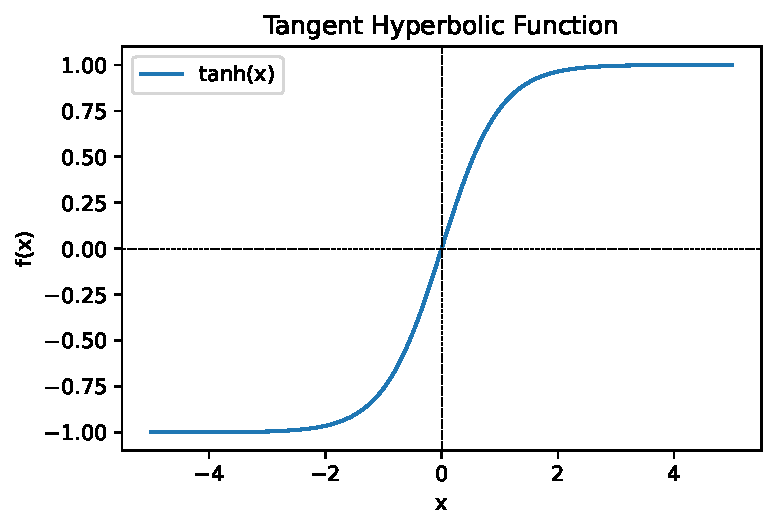
\includegraphics[keepaspectratio]{pr_03_files/figure-pdf/cell-2-output-1.pdf}}

\subsection{4. Minima, Maxima}\label{minima-maxima}

Let
\(f : [-1,2] \to \mathbb{R},\; x \mapsto \exp\!\bigl(x^{3}-2x^{2}\bigr)\)

\begin{enumerate}
\def\labelenumi{(\alph{enumi})}
\item
  Compute (f')
\item
  Plot (f) and (f') with\,R
\item
  Find all possible candidates (x\^{}*) for maxima and minima.
   \emph{Hint:} (\exp) is a strictly monotone function.
\item
  Compute (f'\,')
\item
  Determine if the candidates are local maxima, minima, or neither.
\item
  Find the global maximum and global minimum of (f)
\end{enumerate}

\subsection{5. Taylor Series}\label{taylor-series}

Find the Taylor polynomial of the function (f(x) = \sin(x)) around (x =
0).

\subsection{6. Signed area}\label{signed-area}

What is the signed area between the curve (f(x) = x\^{}2) and the x-axis
on the interval ({[}-1, 1{]})?

\begin{enumerate}
\def\labelenumi{\arabic{enumi}.}
\tightlist
\item
  \(2 - 4x\)
\item
  \(x^2 + 2\)
\item
  \(e^{-x}\)
\item
  \(\sin(x)\)
\end{enumerate}

\subsection{7. Convexity}\label{convexity}

Consider two convex functions (f, g : \mathbb{R} \to \mathbb{R}).

\begin{enumerate}
\def\labelenumi{(\alph{enumi})}
\item
  Show that (f + g : \mathbb{R} \to \mathbb{R},, x \mapsto f(x) + g(x))
  is convex.
\item
  Now, assume that (g) is additionally non‑decreasing, i.e.~(g(y)
  \ge g(x)) for all (x \in \mathbb{R}) and all (y \in \mathbb{R}) with
  (y \textgreater{} x). Show that (g \circ f) is convex.
\end{enumerate}




\end{document}
